\documentclass[a4paper,
               %boxit,        % check whether paper is inside correct margins
               %titlepage,    % separate title page
               %refpage       % separate references
               %biblatex,     % biblatex is used
               keeplastbox,   % flushend option: not to un-indent last line in References
               %nospread,     % flushend option: do not fill with whitespace to balance columns
               %hyphens,      % allow \url to hyphenate at "-" (hyphens)
               %xetex,        % use XeLaTeX to process the file
               %luatex,       % use LuaLaTeX to process the file
               ]{jacow}
%
% ONLY FOR \footnote in table/tabular
%
\usepackage{pdfpages,multirow,ragged2e} %
\usepackage{physics}  % symbols frequent in physics with briefer commands

% CHANGE SEQUENCE OF GRAPHICS EXTENSION TO BE EMBEDDED
% ----------------------------------------------------
% test for XeTeX where the sequence is by default eps-> pdf, jpg, png, pdf, ...
%    and the JACoW template provides JACpic2v3.eps and JACpic2v3.jpg which
%    might generates errors, therefore PNG and JPG first
%
\makeatletter%
	\ifboolexpr{bool{xetex}}
	 {\renewcommand{\Gin@extensions}{.pdf,%
	                    .png,.jpg,.bmp,.pict,.tif,.psd,.mac,.sga,.tga,.gif,%
	                    .eps,.ps,%
	                    }}{}
\makeatother

% CHECK FOR XeTeX/LuaTeX BEFORE DEFINING AN INPUT ENCODING
% --------------------------------------------------------
%   utf8  is default for XeTeX/LuaTeX
%   utf8  in LaTeX only realises a small portion of codes
%
\ifboolexpr{bool{xetex} or bool{luatex}} % test for XeTeX/LuaTeX
 {}                                      % input encoding is utf8 by default
{\usepackage[utf8]{inputenc}}           % switch to utf8

\usepackage[USenglish]{babel}


%
% if BibLaTeX is used
%
% \ifboolexpr{bool{jacowbiblatex}}%
%  {%
% %   \addbibresource{refs.bib}
%   %\addbibresource{biblatex-examples.bib}
%  }{}
\listfiles

%%
%%   Lengths for the spaces in the title
%%   \setlength\titleblockstartskip{..}  %before title, default 3pt
%%   \setlength\titleblockmiddleskip{..} %between title + author, default 1em
%%   \setlength\titleblockendskip{..}    %afterauthor, default 1em

\begin{document}

\title{ONLINE OPTIMIZATION OF SIRIUS NONLINEAR OPTICS}

\author{M. M. S. Velloso\thanks{matheus.velloso@lnls.br}\textsuperscript{1}, M. B. Alves\textsuperscript{1}, L. Liu, X. R. Resende, F. H. de Sá\\ Brazilian Synchrotron Laboratory (LNLS), Campinas, Brazil \\
		X. Huang, SLAC National Accelerator Laboratory, Menlo Park, USA \\
		\textsuperscript{1}also at Gleb Wataghin Institute of Physics, University of Campinas, Campinas, Brazil 
}
	
\maketitle
%
\begin{abstract}
SIRIUS is the 4th generation storage ring-based synchrotron light source built and operated by the Brazilian Synchrotron Light Laboratory (LNLS). Beam accumulation at SIRIUS storage ring occurs in an off-axis scheme, using a nonlinear kicker (NLK), for which the efficiency depends on a sufficiently large dynamic aperture (DA). 
%During the commissioning phase, the lattice configurations found by optimization of the model's DA and energy acceptance were implemented and rendered the machine an average injection efficiency of 85\%. DA measurements also indicated a smaller aperture than predicted by the model, signaling the necessity of further optimization of the machine. 
This work reports on the application of online optimization using the Robust Conjugate Direction Search (RCDS) algorithm on SIRIUS sextupoles, which resulted in improvements to injection efficiency (IE) and DA in three different machine working tunes. 
\end{abstract}

\section{INTRODUCTION}
At SIRIUS storage ring, the injected beam is delivered at $x=-8.4~\unit{mm}$ where it is kicked by the NLK and captured into the ring acceptance. During the design phase, tracking simulations for this setup predicted a 99\% IE \cite{Liu:IPAC2016-THPMR011}, considering a horizontal dynamic aperture of $-9~\unit{mm}$  estimated from the model with the optimized nonlinear lattice and realistic errors \cite{deSá:IPAC2016-THPMR012}.  The corresponding sextupole settings were implemented in the machine during commissioning and currently renders an IE of about 85\%, with a large variability of $~\pm8\%$. With the start of operations with top-up injection in March 2023, efforts to increase the DA to achieve a high and reliable (repeatable) IE were intensified. 

Following the experiences from other synchrotron facilities \cite{Huang:2015, Liuzzo:IPAC2016-THPMR015, Olsson:IPAC2018-WEPAL047, yang:ipac2022-tupopt064}, online optimization was applied to SIRIUS storage ring to improve the ring dynamic aperture. The experiments were carried using the RCDS algorithm \cite{Huang:2013}, with the IE as objective function to be maximized upon changes in SIRIUS sextupole families strengths. The lattice was optimized in the nominal working point (WP) with horizontal and vertical tunes of $(49.08, 14.14)$, as well as in the $(49.20, 14.25)$ and $(49.16, 14.22)$  WPs, which throughout this text will be referred to as WPs 1, 2 and 3, respectively. A new WP with higher fractional betatron tunes is of interest to improve the orbit stability.

\section{SIRIUS NONLINEAR LATTICE}
 SIRIUS storage ring consists on a 20-cell five-bend-achromat (5BA) lattice 
 comprising a 5-fold symmetric configuration with alternating high and low horizontal betatron functions. A superperiod consists of one high-beta and 3 low-beta sections: A-B-P-B. The B and P low-beta sections are identical as far as first order optics is concerned; but their sextupoles are different. There are 6 achromatic sextupole families: SFA0, SDA0, SFB0, SDB0, SDP0, SFP0 and 15 chromatic families: SDA1, SFA1, SDA2, SFA2, SDA3, SDB1, SFB1, SDB2, SFB2, SDB3, SFP1, SDP1, SFP2, SDP2, SDP3. More details on SIRIUS lattice can be found in ref. \cite{Liu:IPAC2016-THPMR013}.

\section{OPTIMIZATION EXPERIMENTS}

\subsection{Optimization in Working Point 1}
The RCDS objective function was the average IE of five injection pulses at $2~\unit{Hz}$, with a noise sigma of $\sigma \approx 1\%$. The beam was injected with a horizontal offset larger than the usual so the IE would drop to $30$-$40\%$, giving room for improvements. The on-axis dipole kicker (DipK), which is immediately upstream the NLK \cite{Liu:IPAC2016-THPMR011}, was used to capture the injected beam. The motivation to use the DipK is that its field profile should be less sensitive to injection conditions variations than the NLK field. In this way, variations of IE should be mainly related to changes in the DA.

The optimization knobs consisted of the 6 achromatic sextupole families and linear combinations of the chromatic families. Families SFP1 and SFB1 were not included as knobs since they operate close to their upper limit of strength, where hysteresis effects become significant.  Families SDA1, SFA1, SDA2, SDA3, SFA2 were varied independently, while the constrained pairs SDB1 \& SDP1, SDB2 \& SDP2, SFB2 \& SFP2, SDB3 \& SDP3 formed other 4 knobs, resulting in a 9-dimensional search space composed by chromatic sextupoles. The 7-dimensional null space of the chromaticity response matrix with respect to changes in the 9 knobs was calculated using the SIRIUS model and the right-singular vectors spanning it, i.e., those associated with vanishing singular values, were used as knobs. The resulting parameter space consisted on 13 knobs. 

With this setup, three optimization runs were performed. In run 1, RCDS improved the IE from $\sim40\%$ to $\sim80\%$. Starting from the best configuration found, the IE was intentionally worsened by further increasing the horizontal offset and another run was started, taking the IE from $\sim60\%$ to $\sim70\%$. The same procedure was repeated for run 3, with the difference that the machine magnets were standardized prior to applying the best solution. In run 3, IE was optimized from $\sim30\%$ to $\sim60\%$.
 
% runs 1, 2 and 3 are generic names I'm using for the paper only. They correspond to data from friday, february 24. 
% Run 1 consits on the optimization files `rcds_run4_13knobs_dipole_kicker.pickle` + `rcds_run4_13knobs_dipole_kicker_second.pickle` objective history
% Run 2 consists on the file `rcds_run4_13knobs_dipole_kicker_fifth.pickle`
% Run 3 consists on `rcds_run5_13knobs_dipole_kicker.pickle`
\begin{figure}[!h]
   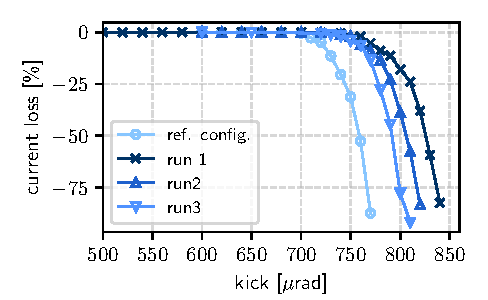
\includegraphics[width=\columnwidth]{WEPL087_f1.pdf}
   \caption{Current losses vs. horizontal dipole kick for the ref. config. and for the RCDS solutions at WP 1.}
   \label{fig:loss_kicks}
\end{figure}
For each one of the best configurations found during runs 1, 2 and 3 and also for the reference configuration (ref. config.), turn-by-turn (TbT) BPM data of the stored beam kicked with the horizontal dipolar kicker were acquired. The DCCT current monitor allowed the determination of the current losses as a function of the horizontal kicks, which is shown by Figure~\ref{fig:loss_kicks}. 
TbT data also allowed for the reconstruction of the $(x,x^\prime)$ phase space of the beam under the influence of the kicks. Using two BPMs at the ends of an empty ID straight section, the position and angle of the beam were determined at each turn. 
Figure~\ref{fig:oldtunes_phase} shows the measured phase spaces for the ref. config. and the best configurations found during run 1, 2, and 3, at the fifth straight section (SA05), which is a high-beta section with identical optics to the injection point. In the measurement, the beam was under the influence of kicks rendering approximately the same current loss of $12\%$.

\begin{figure}[!h]
    \centering
    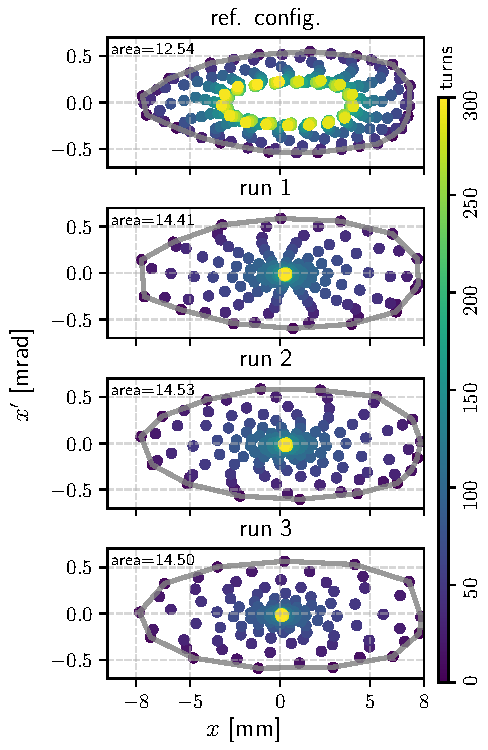
\includegraphics[width=\columnwidth]{WEPL087_f2.pdf}
    \caption{Measured phase space at SA05 high-beta straight section for the ref. config. and the best RCDS configurations of runs 1, 2 and 3 in WP 1. Color-map indicates the turns. The areas are in $\unit{mm}~\unit{mrad}$. The beam was being kicked horizontally at $730~\unit{\micro rad}$ in the ref. config, $790~\unit{\micro rad}$ in run 1, $780~\unit{\micro rad}$ in run 2, and $770~\unit{\micro rad}$, in run 3. Loss rates of  $12\%, 11\%, 13\%$ and $13\%$.} 
    \label{fig:oldtunes_phase}
\end{figure}
Table~\ref{table1} compiles the IE achieved for each configuration during off-axis NLK injection in normal injection conditions ($x\approx -8.5~\unit{mm}$, $x^\prime\approx 0 $). 
Interestingly, the configuration with the largest kick resilience, that of run 1, is not the one with the largest phase space area and IE performance. This could be explained if the phase space deformations of the ellipse at the kicker location for this sextupole setting resulted in a larger $x^\prime/x$ ratio, which would account for a larger kick acceptance and the worse injection performance compared to run 2. 

Lifetime at $60~\unit{mA}$ with uniform filling and bunch-by-bunch (BbB) feedback loop closed was measured at $20~\unit{hr}$ for run 2 best configuration. Lifetime at the same conditions for the reference configuration is $21~\unit{hr}$. No significant chromaticity changes were observed: $(2.33, 2.53)$ in ref. config. vs. $(2.24, 2.39)$ in run 2 best solution.  
\begin{table}[!h]
\centering
\caption{Injection efficiency (IE) of the initial configurations and the best configurations of the optimization runs in WPs 1 and 2.} 
\begin{tabular}{cccc}
\toprule
\multicolumn{2}{c}{working point 1}         & \multicolumn{2}{c}{working point 2}                \\ \midrule
configuration & IE $[\%]$ & configuration        & IE $[\%]$ \\ \hline
ref. config.  & $88\pm8$                & initial              & $51\pm1$                \\
run 1         & $91\pm1$                & run 1                & $79\pm3$                \\
run 2         & $98\pm1$                & run 2                & $65\pm1    $                \\
run 3         & $87\pm3$                & \multicolumn{1}{l}{} & \multicolumn{1}{l}{}        \\ \hline
\end{tabular}

\label{table1}
\end{table}


\subsection{Optimization in Working Point 2}
 SIRIUS nominal WP has low fractional parts, which amplifies orbit distortions. In recent orbit stability studies, the $(49.20, 14.25)$ point was characterized and the improvement in orbit stability was confirmed. The configuration in this WP was loaded in the machine for nonlinear lattice optimization and the initial IE was $\sim50\%$. Two optimization runs were carried out. In run 1, the same knobs used in the previous three runs at WP 1 were used. In run 2, the constraint in the B and P families was removed, resulting in 13 chromatic knobs. Out of these, 11 knobs living in the chromaticity response matrix null space were used alongside the 6 achromatic families, totaling 17 knobs. 
 
 During run 1, IE was optimized from $20\%$ to $60\%$, worsened back to $20\%$ and optimized again to $40\%$. Lastly, it was optimized from $25\%$ to $30\%$. From the best configuration  of run 1, run 2 was started with the 17-knob setup. The initial IE of $35\%$ reached $65\%$, was worsened to $20\%$ and optimized to $40\%$. Lastly, the IE was optimized from $20\%$ to $30\%$, approximately.

TbT BPM data of the kicked stored beam  in the initial configuration and in each run's best solution was acquired and allowed the determination of current losses vs. kicks, shown in Fig.~\ref{fig:loss_kicks_newtunes}, and the reconstruction of phase space, shown in Fig. ~\ref{fig:newtunes_phase}. Table~\ref{table1} compiles injection efficiencies achieved for the configurations in the new tunes during nominal off-axis injection. The configuration found during run 1 rendered the best IE, the largest kick resilience, a larger lifetime than the initial configuration ($21~\unit{hrs}$, run 1 vs. $18~\unit{hrs}$, initial, at $60~\unit{mA}$), and the largest phase-space area increase.
\begin{figure}[!h]
   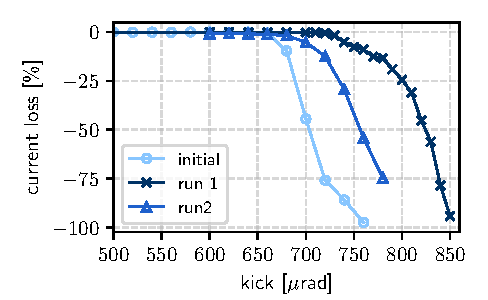
\includegraphics[width=\columnwidth]{WEPL087_f3.pdf}
   \caption{Current losses vs. horizontal dipole kick for the initial configuration and the RCDS solutions at WP 2.}
   \label{fig:loss_kicks_newtunes}
\end{figure}

\begin{figure}
   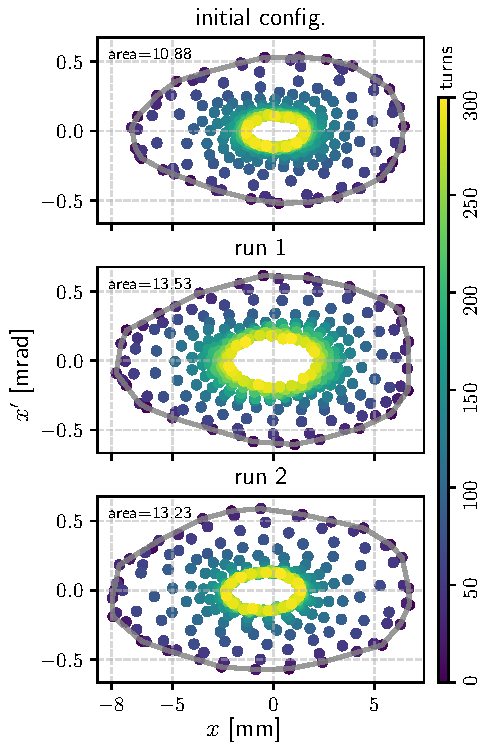
\includegraphics[width=\columnwidth]{WEPL087_f4.pdf}
   \caption{Measured phase space at SA05 high-beta straight section for the initial configuration and the best RCDS configurations of runs 1 and 2 in WP 2. Color-map indicates the turns. The areas are in $\unit{mm}~\unit{mrad}$. The beam was being kicked horizontally at $680~\unit{\micro rad}$, for the initial configuration, $770~\unit{\micro rad}$ for run 1, and at $720~\unit{\micro rad}$ for run 2. Loss rates of $10\%$, $12\%$ and $12\%$, respectively}
   \label{fig:newtunes_phase}
\end{figure}

\subsection{Optimization in Working Point 3}
In the $(49.16, 14.22)$ WP , the knobs consisted on the achromatic families plus the SDA1, SDB1, SDP1, SDA3, SDB3, SDP3 and SFA1 families. The scheme for changing knobs while keeping chromaticity constant was different: RCDS freely varied the 13 optimization knobs. The chromaticity changes due to the knobs changes were anticipated using the machine model, and a set of ``correction" families (SDA2, SDB2, SDP2, SFA2, SFB2, and SFP2) were used to cancel them, so that the strengths applied to the machine rendered no changes in chromaticity.  

Two optimization runs were carried out, starting from sextupole settings of the reference configuration. In run 1, starting from about $20\%$ IE, a configuration rendering $83\%$ IE was found and loaded into the machine. The beam's horizontal offset during injection was increased to worsen the IE and run 2 was started from $48\%$ IE. A configuration rendering $80\%$ IE was found and loaded into the machine, rendering an IE of $93\pm3\%$ in normal off-axis injection conditions. Lifetime at $60~\unit{mA}$ was measured at $19.5~\unit{hrs}$. Kick resilience, phase-space and chromaticity were not yet measured by the time of writing. Orbit stability improvements were confirmed by the orbit integrated spectrum density, which decreased by a factor of approximately 2 \cite{Liu:IPAC23-WEOGA2}.

\section{CONCLUSIONS}
RCDS optimization was applied to SIRIUS storage ring nonlinear lattice to increase the DA and IE in three WPs. In WP 1, IE was optimized to $98\%$ with a 1-hour reduction in lifetime, while, in WP 2, starting from about $50\%$, an IE of $79\%$ was achieved with no changes to lifetime compared to the reference configuration. In WP 3, an IE of $93\%$ was reached with a small reduction in beam lifetime. Despite not being fully characterized, this WP and the RCDS-optimized sextupole settings were set as SIRIUS new reference configuration for top-up operations during user's beam.
\section{ACKNOWLEDGEMENTS}
M. M. S. Velloso is supported by the São Paulo Research Foundation (FAPESP) via grant \#2022/04162-4. 
%
% only for "biblatex"
%
% \ifboolexpr{bool{jacowbiblatex}}%
% 	{\printbibliography}%
% 	{%
	% "biblatex" is not used, go the "manual" way
	
	%\begin{thebibliography}{99}   % Use for  10-99  references
	\begin{thebibliography}{9} % Use for 1-9 references
	
        
%     \bibitem{Alves:IPAC21-MOPAB260}
%        M. B. Alves,
%        \textquotedblleft{Optics Corrections with LOCO on Sirius Storage Ring}\textquotedblright,
%        in \emph{Proc. IPAC’21}, Campinas, Brazil, May 2021, pp. 825--828.
%        \url{doi:10.18429/JACoW-IPAC2021-MOPAB260} 

    \bibitem{Liu:IPAC2016-THPMR011}
        L. Liu, \emph{et al.},
       \textquotedblleft{{I}njection {D}ynamics for {S}irius {U}sing a {N}onlinear {K}icker}\textquotedblright,
       in \emph{Proc. IPAC’16}, Busan, Korea, May 2016, pp. 3406--3408.
       \url{doi:10.18429/JACoW-IPAC2016-THPMR011} 
 
    \bibitem{deSá:IPAC2016-THPMR012}
        F. H. de Sá, L. Liu, X. R. Resende,
       \textquotedblleft{{O}ptimization of {N}onlinear {D}ynamics for {S}irius}\textquotedblright,
       in \emph{Proc. IPAC’16}, Busan, Korea, May 2016, pp. 3409--3412.
       \url{doi:10.18429/JACoW-IPAC2016-THPMR012}

    \bibitem{Liu:IPAC2016-THPMR013}
       L. Liu, X. R. Resende, and F. H. de Sá,
       \textquotedblleft{A New Optics for Sirius}\textquotedblright,
    %  in \emph{Proc. IPAC2016}, pp. 3413--3416,
     in \emph{Proc. IPAC'16}, Busan, Korea, May 2016, pp. 3413--3416.
    %  in \emph{Proc. 7th Int. Particle Accelerator Conf. (IPAC'16)}, 
    %  Busan, Korea, May 2016, paper THPMR013, pp. 3413--3416,
    %  ISBN: 978-3-95450-147-2,
    %  \url{http://jacow.org/ipac2016/papers/thpmr013.pdf},
       \url{doi:10.18429/JACoW-IPAC2016-THPMR013}, 2016.
           
	\bibitem{Huang:2013}
		X. Huang, J. Corbett, J. Safranek, J. Wu,
		\textquotedblleft{An algorithm for online optimization of accelerators}\textquotedblright,
		\emph{Nucl.  Instr. Meth.}, vol 726, pp. 77--83, 2013.
        % \url{https://doi.org/10.1016/j.nima.2013.05.046} 
        \url{doi: 10.1016/j.nima.2013.05.046}

    \bibitem{Huang:2015}
		X. Huang, J. Safranek,
		\textquotedblleft{Online optimization of storage ring nonlinear beam dynamics}\textquotedblright,
		\emph{Phys. Rev. ST Accel. Beams}, vol 18, p. 18.
        \url{doi: 10.1103/PhysRevSTAB.18.084001} 
 
    \bibitem{Liuzzo:IPAC2016-THPMR015}
        S. M. Liuzzo, \emph{et al.},
        \textquotedblleft{RCDS Optimizations for the ESRF Storage Ring}\textquotedblright,
        in \emph{Proc. IPAC’16}, Busan, Korea, May 2016, pp. 3420--3423.
       \url{doi:10.18429/JACoW-IPAC2016-THPMR015}   
    
    \bibitem{Olsson:IPAC2018-WEPAL047}
       D. K. Olsson,
       \textquotedblleft{Online Optimisation of the MAX IV 3 GeV Ring Dynamic Aperture}\textquotedblright,
    % --- abbreviated form (published paper) - JACoW template Feb 2018 ---
       in \emph{Proc. IPAC'18}, Vancouver, BC, Canada, Apr. 2018, pp. 2281--2283.
       \url{doi:10.18429/JACoW-IPAC2018-WEPAL047}
    % --- complete form (published paper) - JACoW template Feb 2018 ---
    %  in \emph{Proc. 9th International Particle Accelerator Conference (IPAC'18)}, Vancouver, BC, Canada, Apr. 4,,
    %  pp. 2281--2283, \url{doi:10.18429/JACoW-IPAC2018-WEPAL047}
    % --- additional material ---
    %  ISBN: 978-3-95450-184-7, \url{http://jacow.org/ipac2018/papers/wepal047.pdf}
    
    \bibitem{yang:ipac2022-tupopt064}
        X. Yang, \emph{et al.},
       \textquotedblleft{Online Optimization of NSLS-II Dynamic Aperture and Injection Transient}\textquotedblright,
        in \emph{Proc. IPAC'22}, Bangkok, Thailand, Jun. 2022, pp. 1159--1162.
    % --- complete form (published paper) - JACoW template Feb 2018 ---
    %  in \emph{Proc. 13th International Particle Accelerator Conference (IPAC'22)}, Bangkok, Thailand, Jun. 2022, pp. 1159--1162.
       \url{doi:10.18429/JACoW-IPAC2022-TUPOPT064}

       %\cite{Liu:IPAC23-WEOGA2}
    \bibitem{Liu:IPAC23-WEOGA2}
       L. Liu, \emph{et al.},
       \textquotedblleft{Status of SIRIUS operation with users}\textquotedblright,
       presented at the IPAC’23, Venice, Italy, May 2023, paper WEOGA2, this conference. 
    
   
	\end{thebibliography}

% } % end \ifboolexpr
%
% for use as JACoW template the inclusion of the ANNEX parts have been commented out
% to generate the complete documentation please remove the "%" of the next two commands
% 
%\newpage

%\include{annexes-A4}

\end{document}
